% ============================================================
% 1A
% ============================================================

\section{Task 1A: Loop Unrolling and Reordering}

\subsection{Baseline}
The baseline iterates over output dimensions (\texttt{oy}, \texttt{ox}) as the outer loops and kernel dimensions (\texttt{ky}, \texttt{kx}) as the inner loops. Although accesses along \texttt{kx} are contiguous, this order repeatedly traverses overlapping input windows and does not exploit reuse across adjacent output pixels as effectively as the reordered implementation.

\subsection{Motivation}
Loop reordering targets improved spatial cache locality by accessing the input matrix sequentially. Loop unrolling minimizes branch condition checks and index increment overhead, exposing instruction-level parallelism.

\subsection{Design Considerations}
\begin{itemize}
    \item \textbf{Memory access pattern:} Moving \texttt{ox} to the innermost loop ensures contiguous memory fetches (stride of 1).
    \item \textbf{Cache locality:} Kernel values are cached in a register before the innermost loop, reducing L1 fetches.
    \item \textbf{Unrolling factor:} \texttt{ox} was unrolled by a factor of 8 to maximize scalar accumulator use without register spilling, and \texttt{ky}/\texttt{kx} by 2.
\end{itemize}

\subsection{Implementation}
For \texttt{conv\_reorder}, the loop hierarchy was inverted to \texttt{oy} $\rightarrow$ \texttt{ky} $\rightarrow$ \texttt{kx} $\rightarrow$ \texttt{ox}. For \texttt{conv\_unroll}, the innermost spatial loop steps by 8, accumulating in parallel into eight scalar variables, while kernel loops step by 2 with edge-case handling.

\subsection{Experimental Setup}
\begin{table}[H]
\centering
\caption{Task 1A experimental setup}
\begin{tabular}{ll}
\toprule
Parameter & Value \\
\midrule
CPU & Intel x86 \\
Matrix sizes & $512 \times 512$ to $8192 \times 8192$ \\
Kernel sizes & 3, 5, 7, 9 \\
Compiler & GCC (Baseline) \\
\bottomrule
\end{tabular}
\end{table}

\subsection{Results}
\begin{table}[H]
\centering
\caption{Task 1A performance (K=5)}
\begin{tabular}{lccc}
\toprule
Matrix Size & Baseline Time (ms) & Reorder Speedup & Unroll Speedup \\
\midrule
$512 \times 512$ & 2.97 & 1.97$\times$ & 3.80$\times$ \\
$1024 \times 1024$ & 11.69 & 1.98$\times$ & 3.80$\times$ \\
$2048 \times 2048$ & 46.75 & 1.84$\times$ & 3.67$\times$ \\
$4096 \times 4096$ & 188.77 & 1.88$\times$ & 3.83$\times$ \\
$8192 \times 8192$ & 839.46 & 1.77$\times$ & 3.87$\times$ \\
\bottomrule
\end{tabular}
\end{table}

\begin{figure}[H]
    \centering
    \begin{subfigure}{0.48\textwidth}
        \centering
        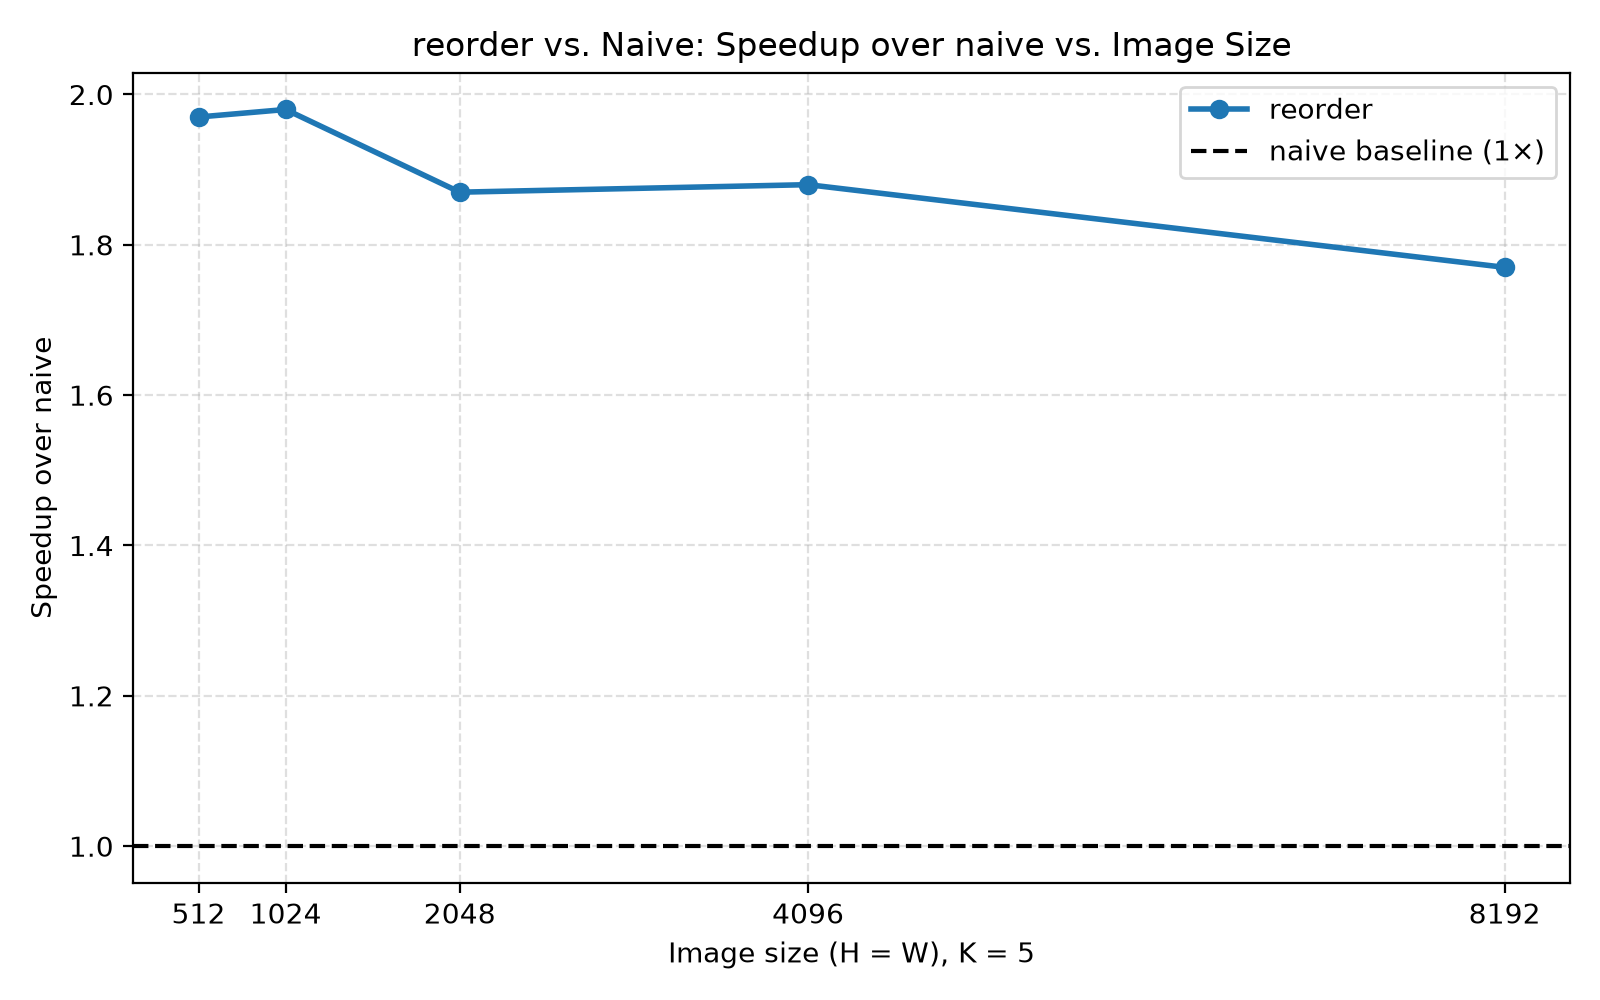
\includegraphics[width=\linewidth]{plots/task1a/reorder_vs_naive_speedup_image_size_k5.png}
        \caption{Reorder: Speedup vs. Image Size ($K=5$)}
        \label{fig:reorder_speedup_size}
    \end{subfigure}
    \hfill
    \begin{subfigure}{0.48\textwidth}
        \centering
        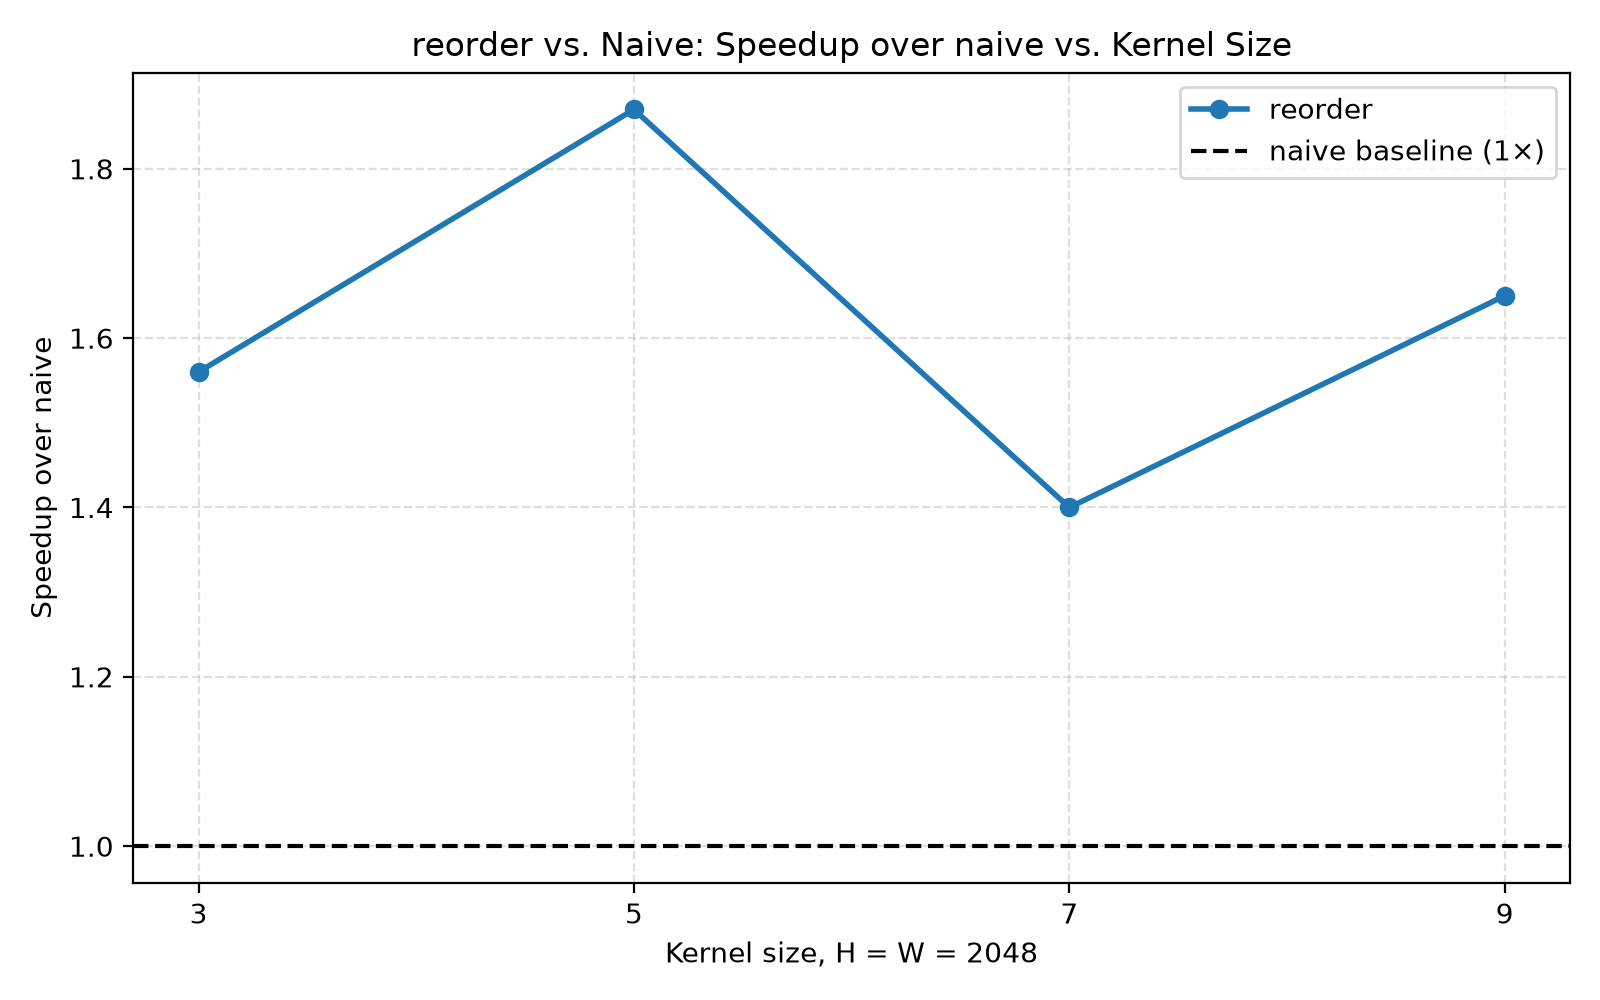
\includegraphics[width=\linewidth]{plots/task1a/reorder_vs_naive_speedup_kernel_size_2048.png}
        \caption{Reorder: Speedup vs. Kernel Size ($2048 \times 2048$)}
        \label{fig:reorder_speedup_kernel}
    \end{subfigure}
    
    \vspace{1em}
    \begin{subfigure}{0.48\textwidth}
        \centering
        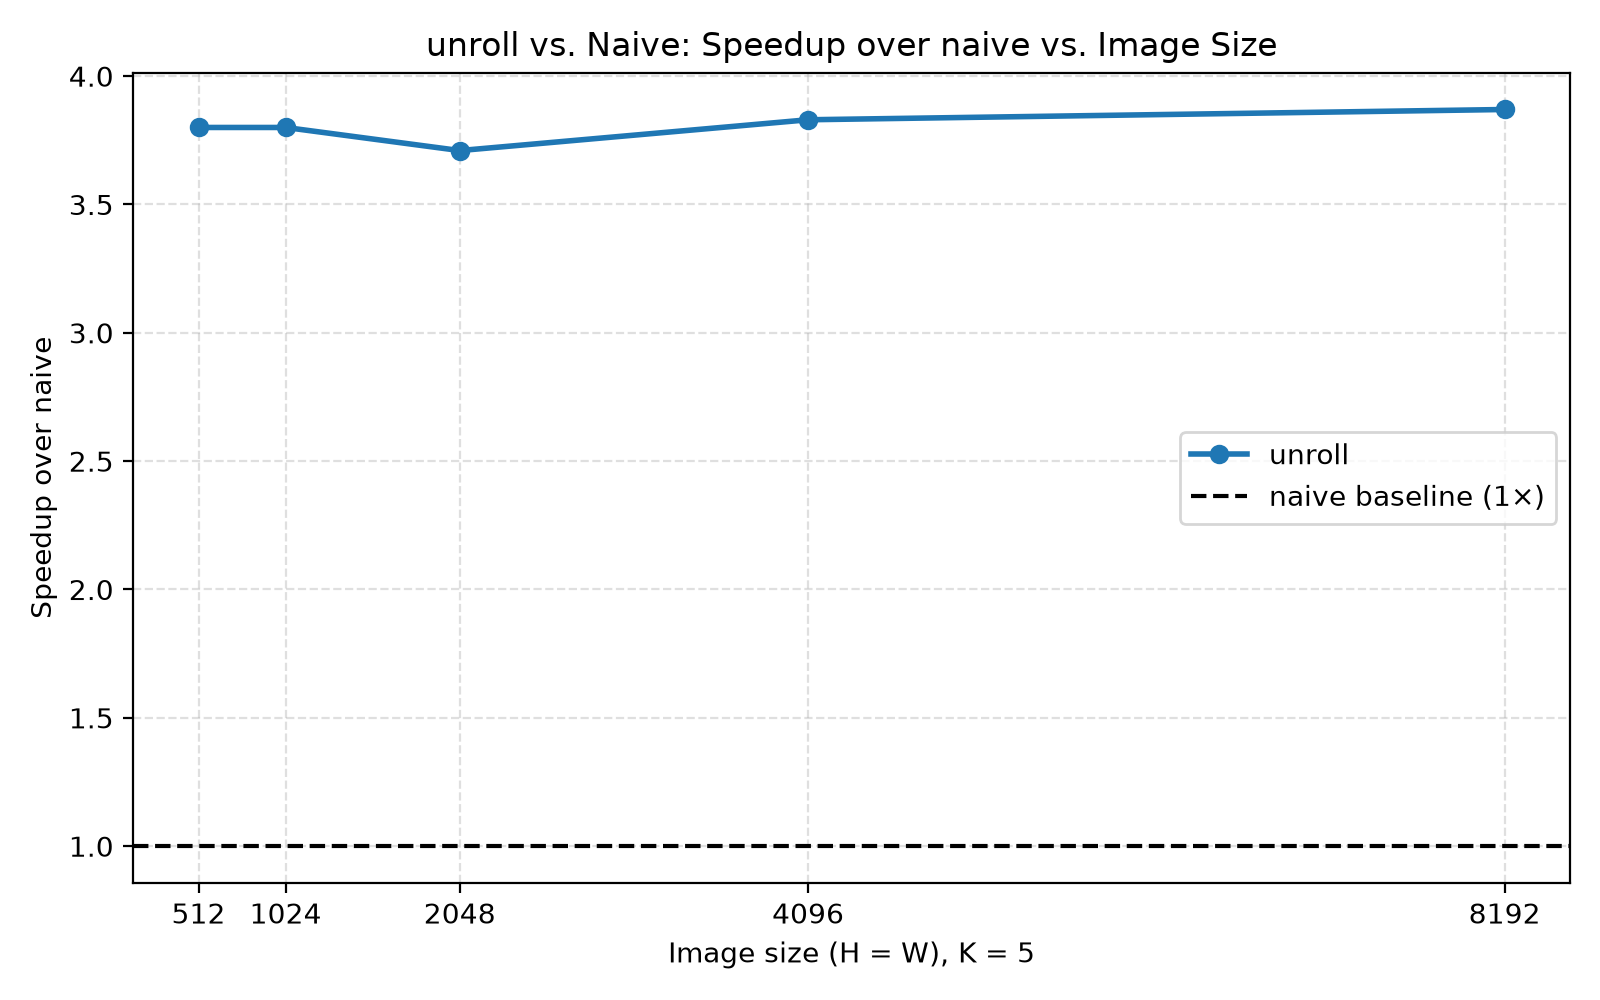
\includegraphics[width=\linewidth]{plots/task1a/unroll_vs_naive_speedup_image_size_k5.png}
        \caption{Unroll: Speedup vs. Image Size ($K=5$)}
        \label{fig:unroll_speedup_size}
    \end{subfigure}
    \hfill
    \begin{subfigure}{0.48\textwidth}
        \centering
        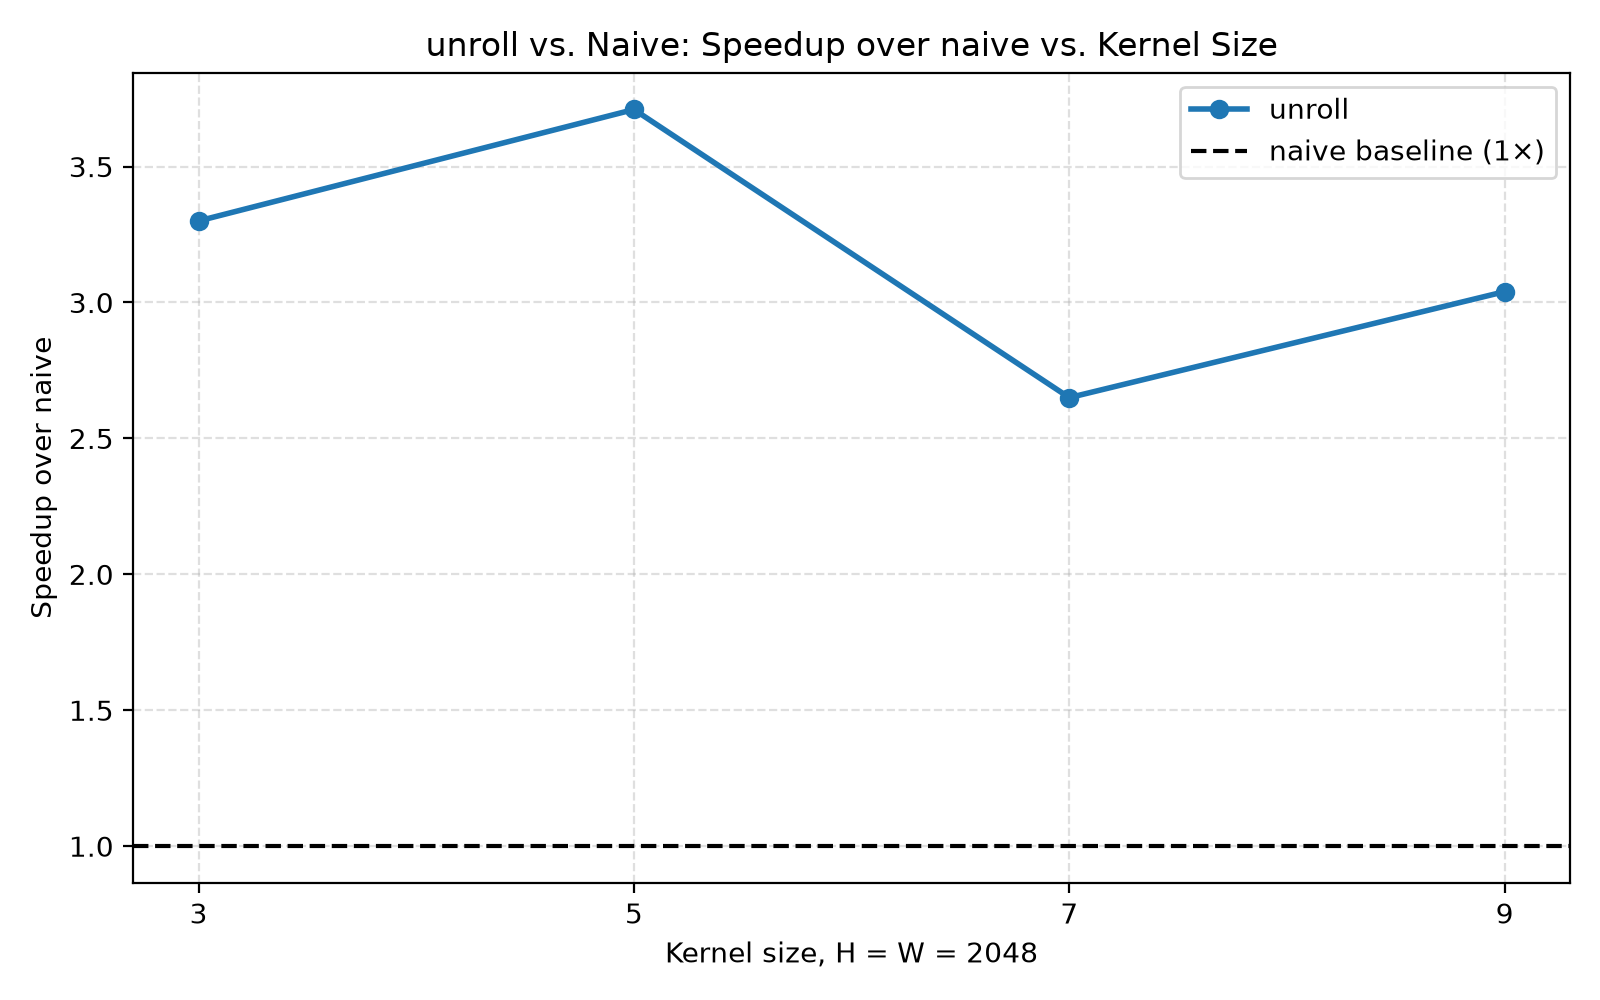
\includegraphics[width=\linewidth]{plots/task1a/unroll_vs_naive_speedup_kernel_size_2048.png}
        \caption{Unroll: Speedup vs. Kernel Size ($2048 \times 2048$)}
        \label{fig:unroll_speedup_kernel}
    \end{subfigure}
    \caption{Speedup performance comparisons against the naive baseline.}
    \label{fig:task1a_speedups}
\end{figure}

\subsection{Analysis}
Reordering yielded nearly a 2$\times$ speedup by making \texttt{ox} the innermost loop and increasing the useful work performed per fetched cache line. Unrolling resulted in an almost 4$\times$ speedup; the gain is consistent with both lower loop-control overhead and greater instruction-level parallelism from the independent accumulators.

As shown in Figure~\ref{fig:task1a_metrics}, unrolling drops instruction counts from $\sim$1.31 billion (naive) to $\sim$359 million (unrolled) for a $512 \times 512$ matrix. 

The total instruction counts for loop reordering remained comparable to the naive baseline but still the difference is significant and the performance is better. This suggests that for this case, we need to take into accoiunt both improved memory-access behavior as well as the instruction count reduction, rather than just one of them. 

\paragraph{Illustrating how Instruction Count Reduction via Reordering}While the primary goal of loop reordering is spatial cache locality, we observed that it also intrinsically reduces the total instruction count by minimizing loop maintenance overhead. This overhead consists of loop variable initialization, bounds checking, and incrementing. 

To illustrate, consider our spatial dimension ($2048$) and kernel dimension ($3$):
\begin{itemize}
    \item \textbf{Naive Ordering (Outer 2048, Inner 3):} The inner loop must be initialized $2048$ times. The outer loop evaluates its condition and increments $2048$ times.
    \item \textbf{Reordered (Outer 3, Inner 2048):} The inner loop is initialized only $3$ times. The outer loop evaluates its condition and increments only $3$ times.
\end{itemize}

By placing the spatial loops (\texttt{ox}) with massive bounds on the inside, and the kernel loops (\texttt{kx}) with tiny bounds on the outside, we drastically reduced the number of times the inner loops had to be set up and torn down. Across a full image convolution, this simple reordering inherently eliminates millions of redundant branch and initialization instructions, further contributing to the overall speedup.

\begin{figure}[H]
    \centering
    \begin{subfigure}{0.48\textwidth}
        \centering
        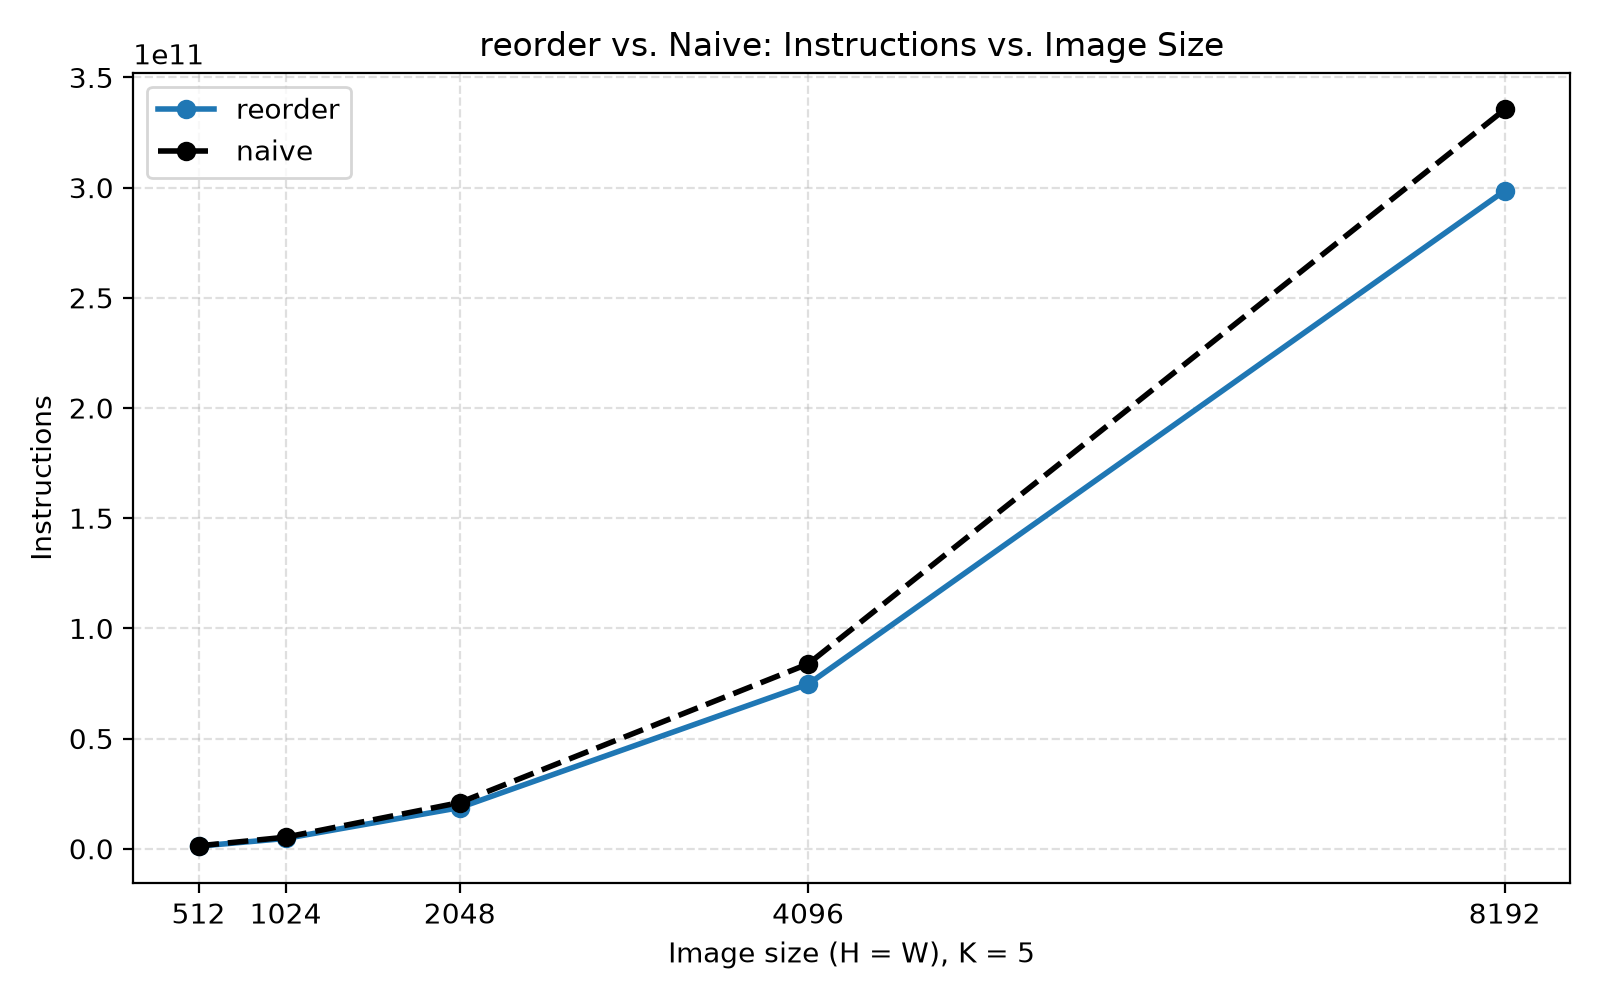
\includegraphics[width=\linewidth]{plots/task1a/reorder_vs_naive_instructions_image_size_k5.png}
        \caption{Reorder: Instructions vs. Image Size ($K=5$)}
    \end{subfigure}
    \hfill
    \begin{subfigure}{0.48\textwidth}
        \centering
        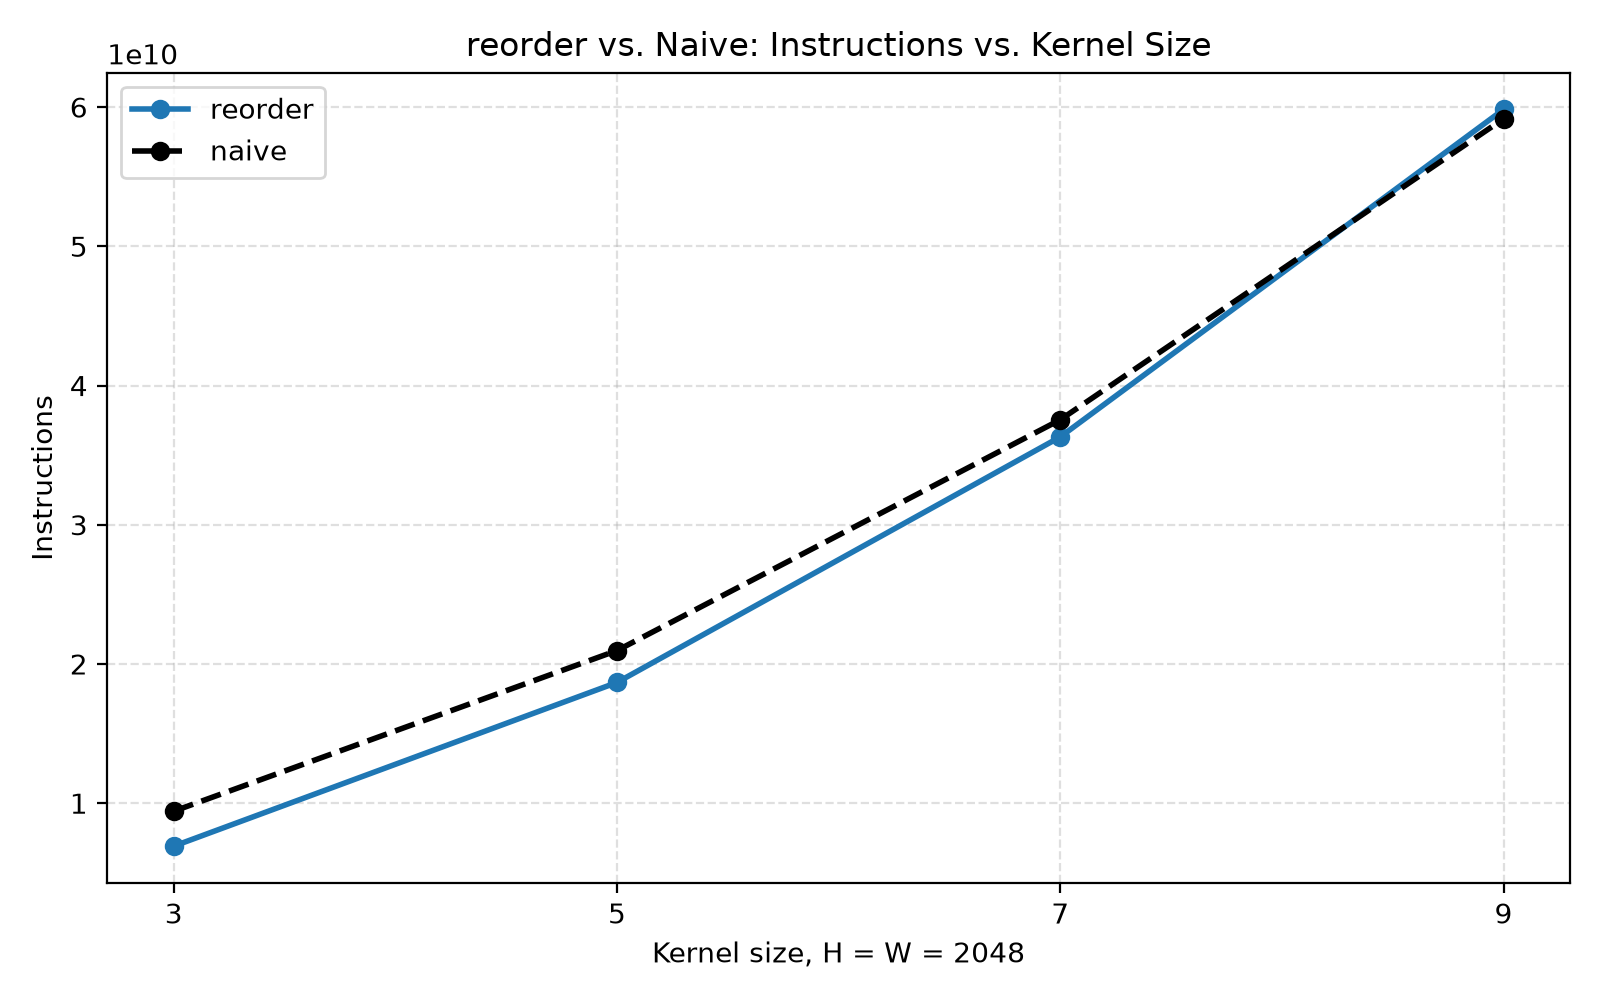
\includegraphics[width=\linewidth]{plots/task1a/reorder_vs_naive_instructions_kernel_size_2048.png}
        \caption{Reorder: Instructions vs. Kernel Size ($2048 \times 2048$)}
    \end{subfigure}
    
    \vspace{1em}
    \begin{subfigure}{0.48\textwidth}
        \centering
        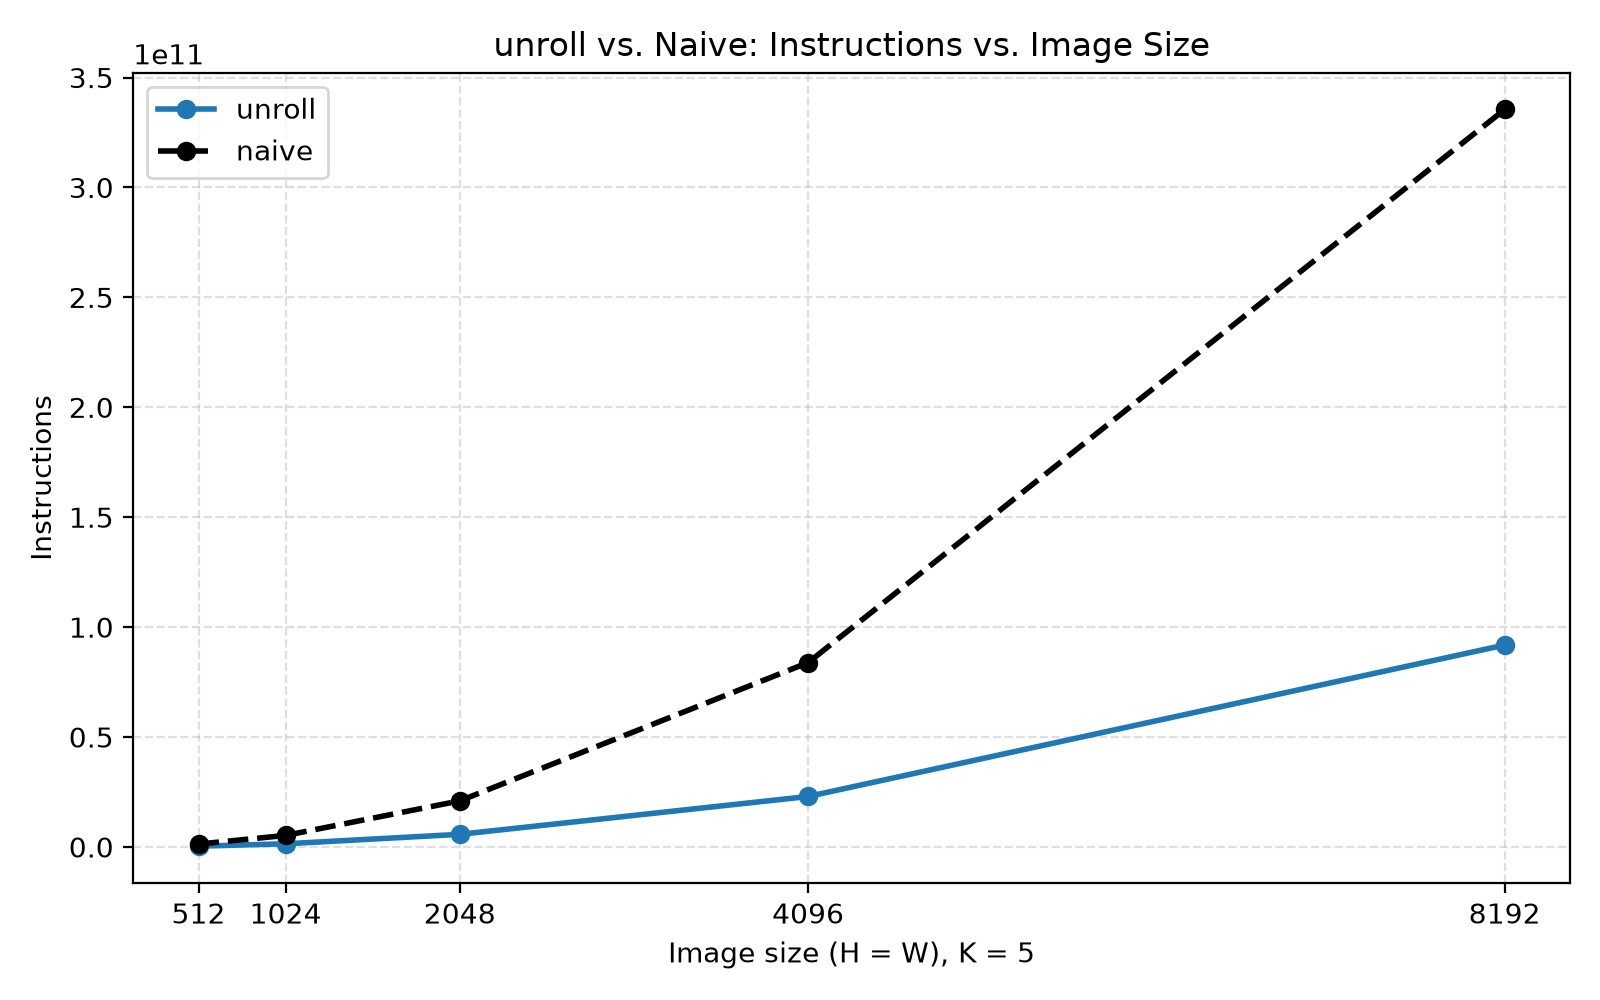
\includegraphics[width=\linewidth]{plots/task1a/unroll_vs_naive_instructions_image_size_k5.png}
        \caption{Unroll: Instructions vs. Image Size ($K=5$)}
    \end{subfigure}
    \hfill
    \begin{subfigure}{0.48\textwidth}
        \centering
        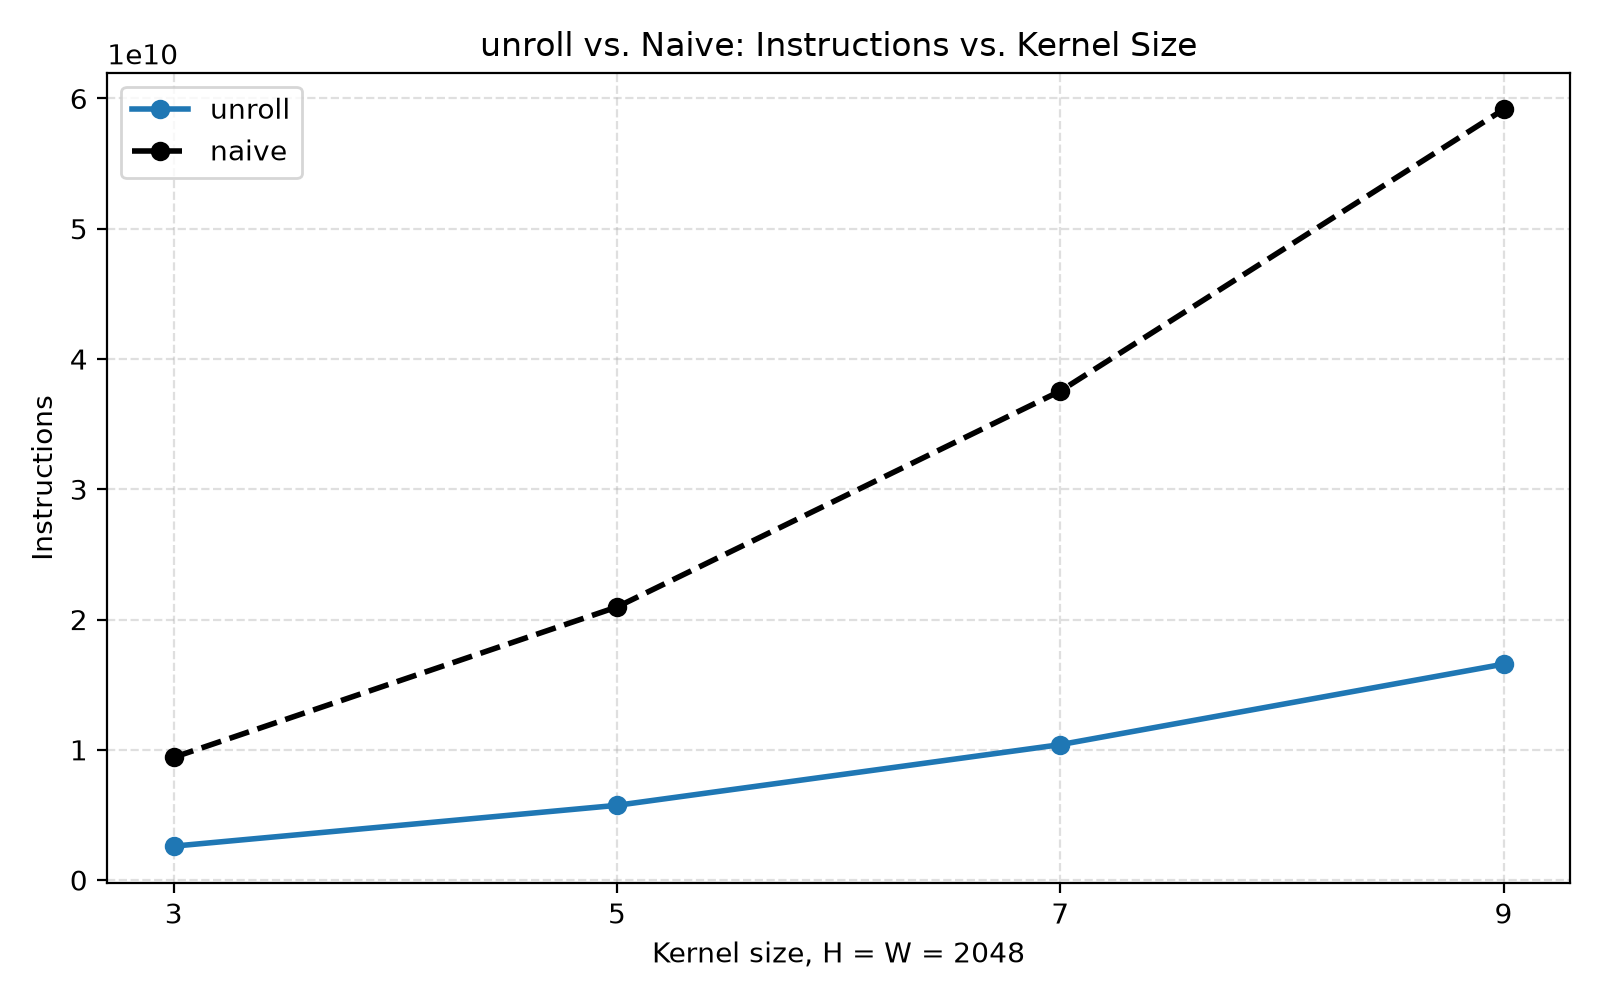
\includegraphics[width=\linewidth]{plots/task1a/unroll_vs_naive_instructions_kernel_size_2048.png}
        \caption{Unroll: Instructions vs. Kernel Size ($2048 \times 2048$)}
    \end{subfigure}

    \vspace{1em}
    \begin{subfigure}{0.48\textwidth}
        \centering
        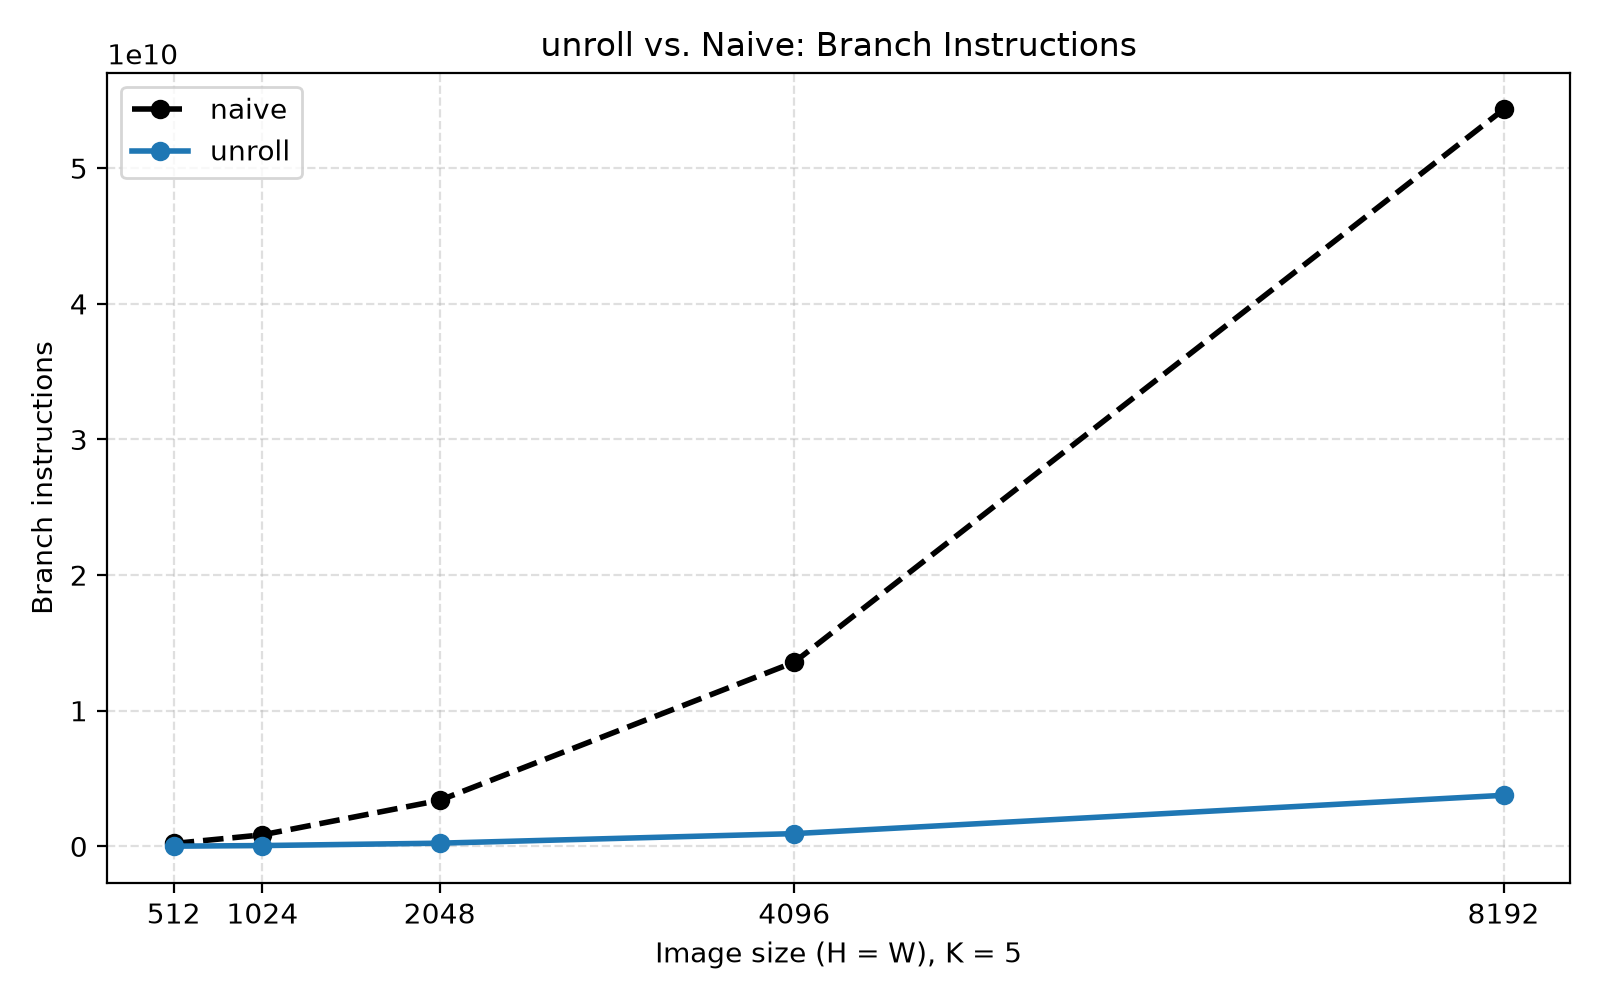
\includegraphics[width=\linewidth]{plots/task1a/unroll_vs_naive_branches_image_size_k5.png}
        \caption{Unroll: Branches vs. Image Size ($K=5$)}
    \end{subfigure}
    \hfill
    \begin{subfigure}{0.48\textwidth}
        \centering
        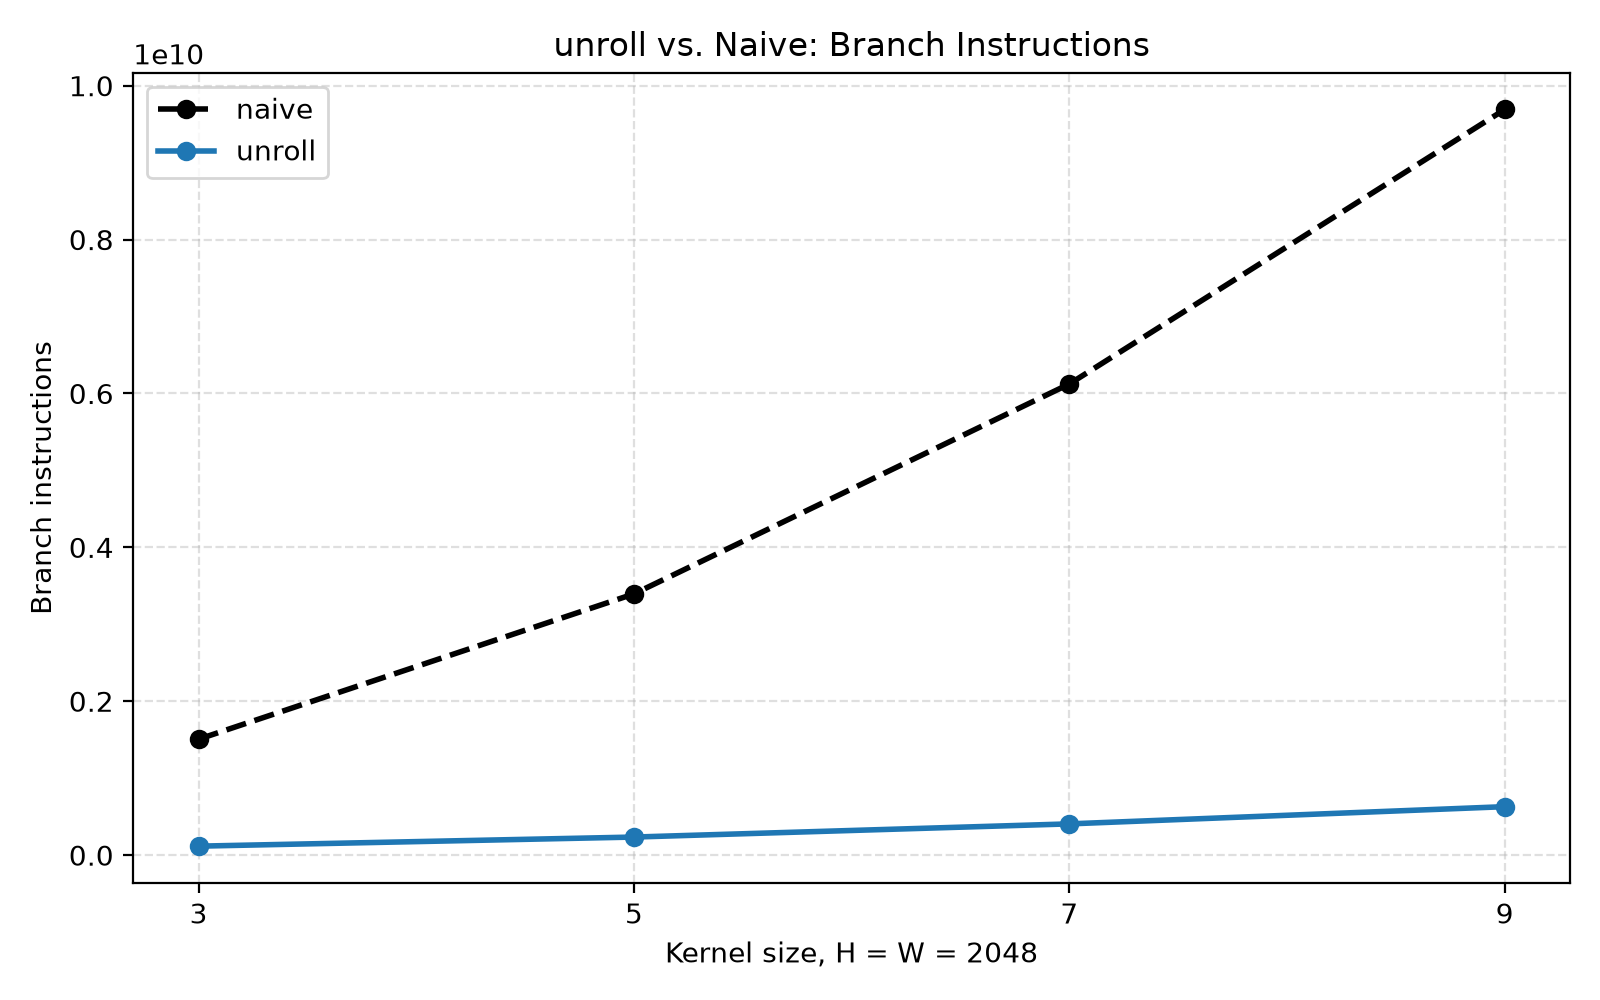
\includegraphics[width=\linewidth]{plots/task1a/unroll_vs_naive_branches_kernel_size_2048.png}
        \caption{Unroll: Branches vs. Kernel Size ($2048 \times 2048$)}
    \end{subfigure}
    \caption{Hardware instruction and branch metrics demonstrating loop overhead reduction.}
    \label{fig:task1a_metrics}
\end{figure}

\subsection{Questions}
\begin{enumerate}
    \item \textbf{What motivated you to make changes to the code?} \\
    To reduce loop-control work and improve reuse across adjacent output pixels; the baseline already has contiguous accesses along \texttt{kx}, but its overall loop order does not expose this reuse as effectively.
    \item \textbf{What considerations did you take into account?} \\
    I prioritized contiguous spatial memory access (reordering) and balanced the unroll factor (8 for spatial width) to fully utilize registers without spilling.
    \item \textbf{How effective were the changes? Which metric was used and why?} \\
    Effective (up to 3.87$\times$ speedup). Execution time was used for raw performance, while instruction counts and branch metrics support the interpretation that unrolling reduces loop overhead and exposes independent work.
\end{enumerate}
